\section{External Architecture}
Two external architectures are described in this section, namely those of the \giraf[] launcher, and the \guicomponents[] library.

\subsection{\giraf[] Launcher}
\label{sec:launcher_architecture}
The external architecture of the launcher can be seen in \autoref{fig:external_architecture}.
\begin{figure}[h]
	\centering
	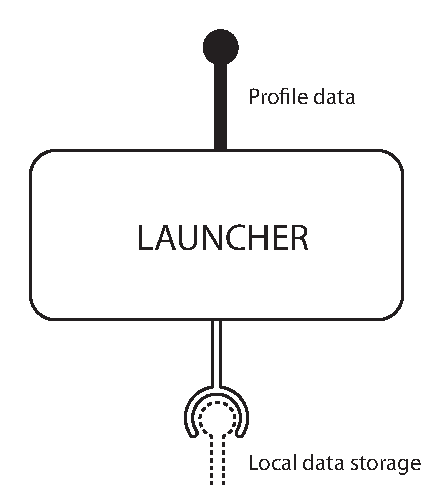
\includegraphics[width=0.5\textwidth]{gfx/external_launcher_architecture.pdf}
	\caption{The external architecture of the \giraf[] launcher.}
	\label{fig:external_architecture}
\end{figure}
The launcher provides two essential services: The ability for users to run, i.e. \textit{launch}, apps, and the provisioning of profile data to these apps. 
The launcher currently allows only \giraf[] apps to be used, but this is by design, as the launcher currently does not support addition and removal of apps. 
The profile data service allows a \guardian[] profile to select a child profile to use a given app with. 
Both the ID of the \guardian[] profile and the child profile is then provided to the app, in order to make it easy for a \guardian[] to switch between different children as needed, while maintaining specific app customizations for different profiles. \newline

The \giraf[] launcher has only one dependancy in the \giraf[] system, namely the Oasis database. 
The launcher is heavily integrated with Oasis, and as such requires the Oasis database to be installed on the device to function. 
Services utilized by the launcher include profile authentication, saving and loading of settings and app integration. 

\subsection{\guicomponents[]}
The \guicomponents[] architecture is designed to be flexible. 
The flexibility is important to keep the \guicomponents[] open and changeable by anyone involved in the development of \giraf[]. 
As such, the only architectural requirement for components that are added to \guicomponents[], is that they should be based on existing Android UI components. 
The philosophy behind this architecture, is that by using existing Android UI components, with a new layout and possible added functionality, the components are already well defined and fully supported in Android. 
The example shown in \autoref{fig:gui_comp_architecture} highlights a possible way of incorporating a component, assuming the need for a customized button: \textit{GButton}. 
\begin{figure}[h]
	\centering
	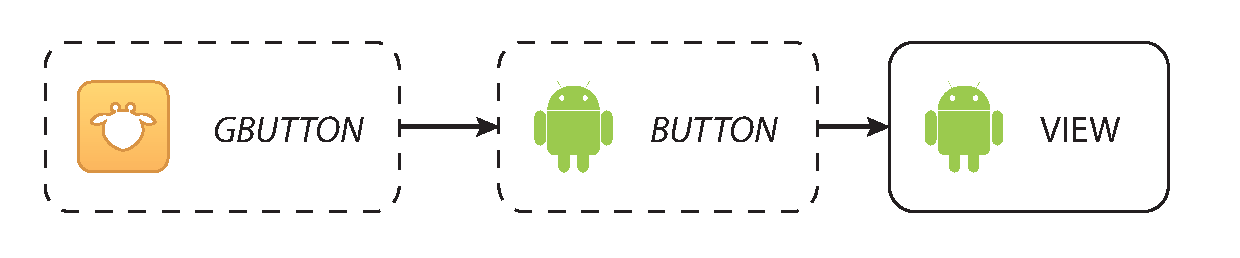
\includegraphics[width=1\textwidth]{gfx/gui_components_architecture.pdf}
	\caption{\guicomponents[] Architecture Example}
	\label{fig:gui_comp_architecture}
\end{figure}